%! Author = Runge
%! Date = 29-12-2023

% Preamble
\documentclass[english,a4paper,compsoc,journal]{IEEEtran}
\overfullrule=10pt
\frenchspacing

% Packages
%! Author = Runge
%! Date = 29-12-2023

\title{Symbolic Parameter Estimation of Continuous-Time Markov Chains}

\author{
\IEEEauthorblockN{Lars Emanuel Hansen}
\IEEEauthorblockA{\textit{dept. of Computer Science} \\
\textit{AAU}\\
Aalborg, Denmark \\
leha20@student.aau.dk}
\and
\IEEEauthorblockN{Daniel Runge Petersen}
\IEEEauthorblockA{\textit{dept. of Computer Science} \\
\textit{AAU}\\
Aalborg, Denmark \\
dpet20@student.aau.dk}\\
\and
\IEEEauthorblockN{Sebastian Aaholm}
\IEEEauthorblockA{\textit{dept. of Computer Science} \\
\textit{AAU}\\
Aalborg, Denmark \\
saahol20@student.aau.dk}
}
%! Author = Runge
%! Date = 29-12-2023

% Packages
\RequirePackage{setup/clrscode4e}
\usepackage{amsmath}
\usepackage{amsthm}
\usepackage{amssymb}
\usepackage{amsbsy}
\usepackage{mathrsfs}
\usepackage{dsfont}
\usepackage{bbold}
\usepackage{booktabs}
\usepackage{tikz}
\usepackage{bbm}
\usetikzlibrary{positioning}
\usetikzlibrary{calc}

\tikzset{%
  zeroarrow/.style = {-stealth,dashed},
  onearrow/.style = {-stealth,solid},
  c/.style = {circle,draw,solid,minimum width=2em,
        minimum height=2em},
  t/.style = {rectangle,draw,solid,minimum width=2em,
        minimum height=2em}
}

% Packages with options set
\usepackage[hidelinks]{hyperref}
\usepackage[textsize=small,obeyDraft]{todonotes}
\usepackage[newfloat]{minted}
\usepackage[backend=biber,
    bibencoding=utf8,
    maxbibnames=20,
    style=ieee,
    citestyle=numeric-comp,
    url=false
]{biblatex}
\usepackage[acronym]{glossaries}

% Package setup
\setlength{\marginparwidth}{2cm} % todonotes width
\setminted{linenos, autogobble, breaklines, fontsize=\footnotesize, style=friendly, xleftmargin=1em, numbersep=5pt}
\addbibresource{bib/main.bib}

% Other setup and options
\newtheorem{theorem}{Theorem}
\newtheorem{definition}{Definition}
\newfloat{algorithm}{htb!}{lop}
\floatname{algorithm}{Algorithm}
\newcommand{\algorithmautorefname}{Algorithm}
\makeatletter
\newcommand*\bigcdot{\mathpalette\bigcdot@{.5}}
\newcommand*\bigcdot@[2]{\mathbin{\vcenter{\hbox{\scalebox{#2}{$\m@th#1\bullet$}}}}}
\makeatother
\makeglossaries


%! Author = Runge
%! Date = 29-12-2023

\newacronym{aau}{AAU}{Aalborg University}

% Document
\begin{document}
    %! Author = Runge
%! Date = 29-12-2023
\IEEEtitleabstractindextext{%
    \begin{abstract}
        This is a placeholder abstract.
        The whole template is used in semester projects at \gls{aau}.
    \end{abstract}
    \begin{IEEEkeywords}
        Formal Verification, Parameter Estimation, Decision Diagram
    \end{IEEEkeywords}
}

    \maketitle
    \IEEEdisplaynontitleabstractindextext

    \section{Introduction}\label{sec:introduction}
%This paper is about improving the runtime of Jajapy - a tool for estimating parameters in parametric models~\cite{goossens1993}.
%Introduce Markov models
Markov models are a class of probabilistic models that are used to describe the evolution of a system over time.
A Markov model has the Markov property, which states that the future behavior of the system depends only on its current state and not on its past history~\cite{markov1962theory}.
This property simplifies analysis by focusing only on the present state, making Markov models especially useful for systems where memory-less behavior is a reasonable assumption.

Markov models are widely used in various fields, such as biology, finance, and computer science, to model systems that exhibit stochastic behavior~\cite{covid19_prism,ciocchetta2009bio, mamon2007hidden,lazowska1984quantitative}.
As such, their analysis has a wide range of applications.

An example of a Markov model, is a simple weather model, if today is sunny, there might be an 80\% chance of sun tomorrow and a 20\% chance of rain.
Similarly, if today is rainy, there might be a 70\% chance of rain tomorrow and a 30\% chance of sun.

%Model checking
Model checking is a technique used to verify the correctness of Markov models by comparing the predictions of the model with observed data.
Model checking is widely used in the verification of Markov models, where the model is analyzed to check if it satisfies certain properties~\cite{clarke1997model}.
It ensures reliability and correctness in critical systems, from traffic controls to industrial automation and communication protocols~\cite{clarke1997model}.
It is also used to check if the model satisfies certain properties, such as reachability, can we reach a desired state and safety properties, can we avoid going a specific sequence of states.

A real world example of model checking is the verification of a traffic light system, where the model is analyzed to check if the traffic lights are working correctly.
For reachability, we can ask: \textit{can a traffic light system always cycle back to green after being red?}.
For safety properties we can ask, \textit{can a traffic light system avoid having both lights green at the same time?}.

There exists several tools for model checking, such as PRISM~\cite{kwiatkowska2011prism} and Storm~\cite{hensel2021probabilistic}, which are widely used in the verification of Markov models.
These tools use symbolic representations to represent the model and perform the operations required for model checking.
The limitation of these tools is that they do not support parameter estimation, which makes them unsuitable for learning the parameters of the model from data.

Parameter estimation is a crucial step in the analysis of Markov models, as the analysis of the model depends on the accuracy of the estimated parameters, particularly when in a timing and probabilistic behaviour~\cite{bacci2023mm}.
Parameter estimation is the process of estimating the parameters of the model from observed data, which is used to make predictions about the system's behavior.

These parameters are used to ensure that the model accurately represents the system's behavior and dynamics and to make accurate predictions about the system's future behavior.
Accurate parameter estimation is essential for making reliable predictions and validating model behavior, with applications ranging from healthcare diagnostics to network security~\cite{bacci2023mm}.

The Baum-Welch algorithm is a widely used method for estimating the parameters of Markov models~\cite{kenny2014deep}.
The algorithm uses the Expectation-Maximization (EM) framework to iteratively update the parameters of the model until convergence~\cite{levinson1983introduction}.
The Baum-Welch algorithm is computationally expensive for large models, as it uses matrices to represent the model, which has a space complexity that grows quadratically with the number of states in the model.
This makes the algorithm computationally expensive for large models, as the memory requirements grow rapidly with the size of the model~\cite{davis2004comparing}.

Addressing these challenges requires innovative techniques, such as symbolic representations, which reduce memory consumption while preserving accuracy.

\subsection{Related Works}\label{subsec:related-works}
%PRISM
PRISM~\cite{kwiatkowska2011prism} is a widely used probabilistic model checker designed to verify the correctness of Markov models.
PRISM has developed a language for specifying models and properties, called the PRISM Language, which is widely used in the field of probabilistic model checking.

When models are specified in the PRISM Language, PRISM can provide a symbolic representation such as \glspl{add} to represent and manipulate the models efficiently, enabling the verification of properties like reachability and safety.

However, PRISM does not support parameter estimation, making it unsuitable for tasks requiring the inference of model parameters from observed data.

%Storm
Storm~\cite{hensel2021probabilistic} is another state-of-the-art probabilistic model checker that shares many similarities with PRISM.
Like PRISM, it can provide a symbolic representations to handle large models efficiently and focuses on verifying properties of Markov models.

It has a parser to read models specified in the PRISM Language, making it easy to use for users familiar with PRISM.
Storm has been optimized for scalability and flexibility, supporting a wide range of model types and verification tasks.

Additionally, Storm is open-source and has a large user base, making it a popular choice for probabilistic model checking.
Despite these strengths, Storm also lacks support for parameter estimation, limiting its utility for learning model parameters from data.

%Jajapy
Jajapy~\cite{reynouard2023jajapy} is a Python-based tool designed for estimating parameters in parametric models using the Baum-Welch algorithm.
It employs a matrix representation of the model and implements the necessary operations for parameter estimation through standard matrix computations without standard matrix libraries.

While accessible and straightforward, Jajapy is hindered by the space complexity inherent in its iterative-based calculation.
This limitation makes it computationally expensive for large-scale models, as memory requirements grow quadratically with the number of states in the system.

%P7 - what is it, what does it do, what are the limitations
SUDD~\cite{p7} builds upon the limitations of Jajapy by introducing a symbolic representation for the forward-backward algorithm.
Specifically, it leverages \glspl{add} to reduce memory consumption and improve the runtime performance of the Baum-Welch algorithm.
By employing \gls{add}-based computations, SUDD provides a significant improvement in scalability, making it feasible to handle larger models.

However, the implementation is limited to a subset of the Baum-Welch algorithm, focusing primarily on forward-backward computations without addressing the full parameter estimation process.

Also the update step in the Baum-Welch algorithm requires SUDD with an explicit state space representation of the model, which limits the scalability of the algorithm.

Our work bridges the gap between parameter estimation tools (e.g.\ Jajapy and SUDD) and model checking tools (e.g.\ PRISM and Storm).
We do this by extending Storm by integrating the Baum-Welch algorithm for with symbolic representations to improve the runtime performance of parameter estimation for Markov models primarily \glspl{hmm}.

This integration of parameter learning with symbolic computation addresses a critical limitation in the current landscape of tools for Markov models.
As a result, Storm can now be used to estimate parameters for \glspl{hmm} from data, enabling the accurate modeling of complex systems.

%In this paper, we extend the work of SUDD by utilizing \glspl{add} in all the steps of the Baum-Welch algorithm to improve the runtime performance of parameter estimation for \gls{hmm}.
%Our approach is to extend Storm with parameter estimation capabilities, by integrating the Baum-Welch algorithm with symbolic representations to improve the runtime performance of parameter estimation for \glspl{hmm}.


% Our approach not only inherits the scalability benefits of \glspl{add} but also implements the complete parameter estimation process.
% Additionally, we compare our implementation with both the original Jajapy, SUDD and an extended version of SUDD using the log-semiring framework, which improves numerical stability in computations.

%By integrating scalable symbolic representations into the full Baum-Welch algorithm, we provide a method that not only estimates parameters efficiently but also enables the accurate modeling of complex systems.


%Model checking
%parameter estimation
%markovian models
%what are they used for (applications)
%what are the challenges

%related works
%what are the current solutions
%P7
%Jajapy
%Prism 
%Storm


% Use the definition LaTeX environment, and base the definitions off of Raphaels paper.


%Describe the field we are in
%Markov models are characterized by the Markov property, which states that the future behavior of the system depends only on its current state and not on its past history. 
%This property makes Markov models well-suited for modeling systems with memoryless behavior, where the future state of the system is independent of its past states given the current state.

%The need for correct parameter estimation in Markov models is crucial for making accurate predictions about the system's behavior and for verifying the validity of the model.
%Probabilistic model checking tools such as PRISM~\cite{kwiatkowska2011prism} and Storm~\cite{dehnert2017storm} are widely used in the verification of Markov models.
%These tools are used to analyze the behavior of the system and to check if the model satisfies certain properties, such as reachability and safety properties.

% For finding the correct properties of the model, the parameters of the model need to be estimated from data, a process known as parameter estimation.
% Parameter estimation is a crucial step in the analysis of Markov models, as it allows us to learn the underlying dynamics of the system and make predictions about its future behavior.
% The Baum-Welch algorithm is a popular method for estimating the parameters for Markov Models~\cite{baum1970maximization}.
% The algorithm uses the Expectation-Maximization (EM) framework to iteratively update the parameters of the model until convergence.
% Normal implementations of the Baum-Welch algorithm uses matrices to represent the model, which has a space complexity that grows quadratically with the number of states in the model. 
% This makes the algorithm computationally expensive for large models, as the memory requirements grow rapidly with the size of the model. 
% The model checkers meantioned before, Storm and Prism, use symbolic data structures such as Algebraic Decision Diagrams (ADD)s to represent the model, which allows them to handle large models efficiently. 
% However, the Baum-Welch algorithm does not take advantage of these symbolic data structures, which limits its scalability for large models.
% This paper aims to improve the runtime of the Baum-Welch algorithm by using a symbolic representation of the model, and use symbolic operations to perform the operations required by the algorithm.

    \section{Preliminaries}\label{sec:preliminaries}
We introduce some preliminary notions and notations, which will be used in the rest of the paper.
The parameter estimation algorithm studied here focuses on \glspl{ctmc}.
We will first introduce the definition of a \gls{ctmc} and \gls{pctmc} then present the Baum-Welch algorithm, which is used to estimate the parameters of a \gls{ctmc}.

\subsection{Continuous-Time Markov Chains}\label{subsec:ctmc}
In stochastic systems, state transitions are governed by two key aspects: timing and transition probabilities.
In \glspl{ctmc}, these aspects are explicitly modeled as separate but interrelated components:

\begin{enumerate}
    \item \textbf{Dwell Time}: The time spent in a state before transitioning to another state.
    This is a random variable governed by an exponential distribution, characterized by the exit rate of the state.
    \item \textbf{Transition Probability}: Once the dwell time elapses, the system transitions to a new state.
    The destination state is determined probabilistically based on the rates of outgoing transitions.
\end{enumerate}
By decoupling these two aspects, \glspl{ctmc} provide a flexible framework for modeling systems where the timing of transitions and the likelihood of transitioning to specific states are influenced by different factors.


\begin{definition}[\gls{ctmc}]
    A \gls{ctmc} is a tuple $\mathcal{M} = (S, \mathcal{L}, \mathscr{l}, R, \pi)$, where:
    \begin{itemize}
        \item $S$ is a finite set of states.
        \item $\mathcal{L}$ is a finite set of labels.
        \item $\mathscr{l}: S \rightarrow \mathcal{L}$ is a labeling function, which assigns a label $\mathcal{L}$ to each state.
        \item $R: S \times S \rightarrow \mathbb{R}_{\geq 0}$ is the rate function.
        The model transitions from state $s$ to state $s'$ with rate $R(s, s')$.
        \item $\pi$ is the initial distribution, the model starts in state $s$ with probability $\pi(s)$.
    \end{itemize}
\end{definition}

\subsubsection{Key Properties}

\begin{enumerate}
    \item The time spent in $s$, known as the dwell time, is exponentially distributed with rate:
    \begin{equation}
        E(s) = \sum_{s' \in S} R(s, s')\label{eq:exitrate} %%TODO: Should we define DTMCs and then add the definition of the transition function/matrix for CTMCs?
    \end{equation}
    \item The probability of transitioning to state $s'$ is given by:
    \begin{equation}
        P(s' \mid s) = \frac{R(s, s')}{E(s)}\label{eq:transition-probability}
    \end{equation}
\end{enumerate}


Transitions are independent of the time spent in the current state.
If there are multiple possible transitions, a race condition occurs, and the first transition to complete determines the next state.


\subsubsection{Discrete Time Markov Chains}
If the dwell time is disregarded or assumed to be uniform across all states, the timing of transitions becomes irrelevant, and the \gls{ctmc} simplifies into a \gls{dtmc}.
In this case, transitions are described by the probabilities $P(s' \mid s)$ of moving to state $s'$ from state $s$.

\subsubsection{Observations in CTMCs}
An execution of the \gls{ctmc} is represented by a sequence of states and dwell times in $\textbf{Paths} \subseteq (S \times \mathbb{R}_{>0} \cup \{\emptyset\})^{\omega}$ where $\omega$ symbolizes infinite execution.
Similarly, an Observation, also called a Trace, is represented by a sequence of labels and dwell times in $\textbf{Observations} \subseteq (\mathcal{L} \times \mathbb{R}_{>0} \cup \{\emptyset\})^{\omega}$.

For a finite observation $\textbf{o} = o_0, o_1, \dots, o_{|\textbf{O}|-1} = (l_0,\tau_0),(l_1,\tau_1),\dots,(l_{|0|-1}), \emptyset \in \textbf{Observations}$:

\begin{itemize}
    \item $l_t \in \mathcal{L}$ is the label observed during the $t$-th transition.
    \item $\tau_t \in \mathbb{R}_{>0} \cup \{\emptyset\}$ is the dwell time observed during the $t$-th transition.
\end{itemize}

if $\tau_t = \emptyset$ for all transitions in a sequence, the sequence is untimed, effectively ignoring dwell times.

%%%%%%%%%%%%%% This text is kind of weird
Intuitively, observations link the observed labels $(l_t)$ and dwell times $(\tau_t)$ to the underlying states of the \gls{ctmc}.
This connection is captured through the likelihood function $\omega_s(t)$, which combines label matching with timing information.

The likelihood of observing an observation $o_t = (l_t, \tau_t)$ in state $s$ is given by the function $\omega_s(i)$, which links the observation to the model's dynamics.
This function ensures that transitions are appropriately weighted by the likelihood of the observed data.

\subsection{Parametric Continuous Time Markov Chains}\label{subsec:parametric-ctmc}
In practice, the rate function $R$ in a \gls{ctmc} is often unknown and must be estimated from observed data.
In systems with complex or uncertain dynamics, \glspl{pctmc} extend \glspl{ctmc} by introducing parameters into the model's rate functions.
These parameters allow for the representation of families of \glspl{ctmc} rather than a single, fixed model.
Like \glspl{ctmc}, \glspl{pctmc} are governed by two key aspects:

\begin{itemize}
    \item \textbf{Dwell Time}: The time spent in a state before transitioning.
    This is determined by the parametric exit rate, which depends on the specific values of the parameters.
    \item \textbf{Transition Probability}: After the dwell time elapses, the system transitions to a new state.
    The probability of transitioning to a particular state is derived from the parametric rates of all outgoing transitions from the current state.
\end{itemize}

For a full description of \gls{pctmc} we refer~\cite{bacci2023mm}.
%The parametric nature of \glspl{pctmc} makes them highly versatile, as they enable the model to adapt to different scenarios or datasets by tuning the parameters.

\begin{definition}[\gls{pctmc}]
    A \gls{pctmc} is a tuple $\mathcal{P} = (S, \mathcal{L}, \mathscr{l}, R, \pi)$, where:
    \begin{itemize}
        \item $S, \mathcal{L}, \mathscr{l}, \pi$ are defined as for \glspl{ctmc}.
        \item $R: S \times S \rightarrow (\mathbb{R}_{\geq 0}^n \rightharpoonup \mathbb{R}_{\geq 0})$ is a parametric transition rate function that maps transitions to polynomial expressions over a vector of parameters $\mathbf{x} = (x_1, \dots, x_n)$.
    \end{itemize}
\end{definition}


In this definition, the rate function under $\mathbf{x}$, $R(s, s'; \mathbf{x})$ determines the rate at which the system transitions from state $s$ to state $s'$ dependent on the parameter values.
Note that the partial function $(\mathbb{R}_{\geq 0}^n \rightharpoonup \mathbb{R}_{\geq 0})(\mathbf{x})$ is the actual evaluation of the rate.


\subsubsection{Key Properties}

\begin{itemize}
    \item For a given state $s$, the parametric dwell time is exponentially distributed with rate:
    \begin{equation}
        E(s; \mathbf{x}) = \sum_{s' \in S} R(s, s'; \mathbf{x}),\label{eq:exitrate-pctmc}
    \end{equation}
    where the sum depends on the current values of the parameters $\mathbf{x}$.
    \item The parametric transition probability is given by:
    \begin{equation}
        P(s' \mid s; \mathbf{x}) = \frac{R(s, s'; \mathbf{x})}{E(s; \mathbf{x})}.\label{eq:transition-probability-pctmc}
    \end{equation}
\end{itemize}

These parametric formulations allow a single \gls{pctmc} to represent a broad class of \glspl{ctmc}, where the specific model instance is determined by fixing the parameter values.

\subsection{Baum-Welch Algorithm}\label{subsec:baum-welch}
The Baum-Welch algorithm is a key method for estimating the probabilities of an \gls{hmm} from observed data. 
The probabilities of an \gls{hmm} are the emission matrix $\omega$, the transition matrix $P$, and the initial distribution $\pi$.
It was chosen as the method for this project due to its ability to estimate the probabilities of a \gls{hmm} without knowing the hidden states that generated the observations, and it is also the standard method for training \glspl{hmm}.
If looking at other Markov models such as \glspl{mc}, the Baum-Welch algorithm can be used to estimate the parameters of the model from observed data, therefore it is a suitable choice for this project, as this can be used to estimate the parameters of other Markov models.
It leverages the Expectation-Maximization (EM) framework and consists of two iterative steps:

\begin{enumerate}
    \item \textbf{Expectation Step (E-step)}: Compute the expected the forward and backward variables, for each state $s$ and time $t$. of the latent variables, which are the unobserved state sequences corresponding to the observations. These variables represent the likelihood of being in state $s$ at time $t$ given the observed data up to time $t$ and the likelihood of observing the remaining data from time $t$ onwards given the state $s$ at time $t$, respectivly. 
    \item \textbf{Maximization Step (M-step)}: Update the model parameters (emission matrix $\omega$, transition matrix $P$, and initial distribution $\pi$) to maximize the likelihood of the observed data, using the expected values computed in the E-step.
    \item Repeat the E-step and M-step until convergence.
\end{enumerate}

The Baum-Welch algorithm is particularly useful for estimating the properbilities of the emission and transition matrices of a HMM, given a set of observations, without knowing the hidden states that generated the observations.

Given a multiset of observations $\mathcal{O}$ and initial parameters $\textbf{x}_0$, the Baum-Welch algorithm estimates the parameters of a \gls{hmm} $\mathcal{P}$ by iteratively improving the current hypothesis $\textbf{x}_n$ using the previous estimate $\textbf{x}_{n-1}$ until a convergence criterion is met.
A hypothesis refers to a specific set of values for the parameters $\mathbf{x}$.

Each iteration of the algorithm produces a new hypothesis, denoted as $\textbf{x}_n$, which is the algorithm's current best guess for the parameter values based on the observed data.
The algorithm consists of three main steps: the forward-backward procedure, the update step, and the convergence criterion.
The Baum-Welch algorithm iteratively refines the parameters until the improvement between successive iterations falls below a predefined threshold.
This is typically evaluated using a convergence criterion such as:

\begin{equation}
    ||l(\textbf{x}_n) - l(\textbf{x}_{n-1})|| < \epsilon\label{eq:convergence-criterion}
\end{equation}

where $\epsilon > 0$ is a small threshold, and $l(\textbf{x}_n)$ denotes the likelihood of the observed data given the parameter values at the $n$-th iteration.

The algorithm stops when the change in parameters is sufficiently small, indicating that the model has converged to a local maximum of the likelihood function.
The parameter estimation procedure is outlined in \autoref{alg:parameter-estimation}.

\begin{algorithm}[htb!]
    \begin{codebox}
        \Procname{$\proc{Estimate-Parameters}(\mathcal{P}, \mathbf{x}_0, \mathcal{O})$}
        \li $\mathbf{x} \gets \mathbf{x}0$
        \li \While $\neg\proc{Criterion}(\mathbf{x}_{n-1}, \mathbf{x}_n)$
        \li \Do $\mathbf{x}_{n - 1} \gets \mathbf{x}_n$
        \li $(\alpha, \beta) = \proc{Forward-Backward}(\mathcal{P}(\mathbf{x}_n), \mathcal{O})$
        \li $\mathbf{x}_n = \proc{Update}(\mathcal{P}(\mathbf{x}_n), \mathcal{O}, \alpha, \beta)$ \End
        \li \Return $\mathbf{x}_n$
    \end{codebox}
    \caption{Parameter estimation procedure~\cite{p7}.}
    \label{alg:parameter-estimation}
\end{algorithm}

Starting with initial parameters $\mathbf{x}_0$, the parameter estimation procedure iteratively improves the current hypothesis $\mathbf{x}_n$ using the previous estimate $\mathbf{x}_{n-1}$ until a specified criterion for convergence is met, the algorithm returns the final estimate $\mathbf{x}_n$.
The specifics of the $\proc{Forward-Backward}$ and $\proc{Update}$ procedures are detailed in \autoref{subsec:forward-backwards_algorithm} and \autoref{subsec:update-algorithm} from~\cite{baum1970maximization}.

\subsection{The Forward-Backward Algorithm}\label{subsec:forward-backwards_algorithm}
For a given \gls{ctmc} $\mathcal{M}$, the forward-backward algorithm computes the forward and backward variables, $\alpha_s(t)$ and $\beta_s(t)$, for each observation sequence $o_0, o_1, \dots, o_{|\mathbf{o}|-1} = \mathbf{o} \in \mathcal{O}$.

The forward variable $\alpha_s(t)$ represents the likelihood of observing the partial sequence $o_0, o_1, \dots, o_t$ and being in state $s$ at time $t$, given the model $\mathcal{M}$:


\begin{equation}
    \alpha_s(t) = l(o_0, o_1, \dots, o_t, S_{t} = s \mid \mathcal{M})
    \label{eq:alpha-recursive}
\end{equation}


The backward variable $\beta_s(t)$ represents the likelihood of observing the partial sequence $o_{t+1}, o_{t+2}, \dots, o_{|\mathbf{o}|-1}$ given state $s$ at time $t$ and the model $\mathcal{M}$:


\begin{equation}
    \beta_s(t) = l(o_{t+1}, o_{t+2}, \dots, o_{|\mathbf{o}|-1} \mid S_{t} = s, \mathcal{M})
    \label{eq:beta-recursive}
\end{equation}


The forward variable $\alpha_s(t)$ and backward variable $\beta_s(t)$ can be computed recursively as follows:


\begin{equation}
    \alpha_s(t) =
    \begin{cases}
        \omega_s(0) \; \pi_s & \text{if } t = 0 \\
        \omega_s(t) \sum_{s' \in S} P_{s's}\alpha_s(t - 1) & \text{if } 0 < t \leq |\mathbf{o}| - 1 \\
    \end{cases}
    \label{eq:forward-recursive}
\end{equation}


\begin{equation}
    \beta_s(t) =
    \begin{cases}
        \mathbbm{1} & \text{if } t = |\mathbf{o}| - 1 \\
        \sum_{s' \in S} P_{ss'} \omega_{s'}(t + 1) \beta_{s'}(t + 1) & \text{if } 0 \leq t < |\mathbf{o}| - 1 \\
    \end{cases}
    \label{eq:backward-recursive}
\end{equation}


Here, $\omega_{s}(t)$ is the likelihood of observing $o_t$ given that the current state at time $t$ is $s$ and the model $\mathcal{M}$, expressed as $\omega_s(t) = l(o_t \mid S_t = s, \mathcal{M})$.
The function $\omega_s(t)$ incorporates observed labels and dwell times into the likelihood computation, linking the data to the model's dynamics.
It ensures the forward-backward algorithm appropriately weights transitions based on their likelihood given the observations.

For \glspl{pctmc}, $\omega_{s}(t)$ is given for some observation $o_t = (l_t, \tau_t)$ by\footnote{Note that $o_{|\mathbf{o}|-1} = (l_{|\mathbf{o}|-1}, \emptyset)$ is always true.}:


\begin{equation}
    \omega_s(t) =
    \begin{cases}
        \lBrack \ell(s) = l_t \rBrack E(s) \; e^{-E_s\tau_t} & \text{if } \tau_t \neq \emptyset \\
        \lBrack \ell(s) = l_t \rBrack & \text{if } \tau_t = \emptyset
    \end{cases}
    \label{eq:omega-pctmc}
\end{equation}


Here:


\begin{itemize}
    \item $\lBrack \ell(s) = l_t \rBrack$ is an indicator function, equal to 1 if the label $\ell(s)$ of state $s$ matches the observed label $l_t$, and 0 otherwise.
    \item $E(s) = \sum_{s' \in S} R(s, s')$ is the total exit rate for state $s$.
\end{itemize}


The forward-backward algorithm computes the forward and backward variables for each state $s$ and time $t$ in the observation sequence $\mathbf{o}$, providing a comprehensive view of the likelihood of the observed data under the model.

\subsection{The Update Algorithm}\label{subsec:update-algorithm}
The update algorithm refines the parameter values of a \gls{pctmc} based on the observed data and the forward and backward variables computed in the forward-backward procedure.
Given the forward and backward variables $\alpha_s(t)$ and $\beta_s(t)$, the update algorithm aims to maximize the likelihood of the observed data by adjusting the parameter values.

The update algorithm iteratively refines the parameter values $\mathbf{x}$ by maximizing the expected log-likelihood of the observed data under the model.
The update step is based on the expected sufficient statistics of the latent variables, which are the unobserved state sequences corresponding to the observations.

\subsubsection{Intermediate Variables}
We need to intermediate variables $\gamma_s(t)$ and $\xi_{ss'}(t)$, $\gamma_s(t)$ represent the expected number of times the model is in state $s$ at time $t$ and $\xi_{ss'}(t)$ represent the expected number of transitions from state $s$ to state $s'$ at time $t$.
These variables are computed as follows:


\begin{equation}
    \gamma_s(t) = \frac{\alpha_s(t) \beta_s(t)}{\sum_{s' \in S} \;(\alpha_{s'}(t) \beta_{s'}(t))}
    \label{eq:gamma}
\end{equation}


In \autoref{eq:gamma}, the numerator is the product of the forward variable $\alpha_s(t)$ and the backward variable $\beta_s(t)$, representing the joint probability of observing the sequence up to time $t$ and the model being in state $s$ at time $t$.
The denominator normalizes the probabilities across all states $s' \in S$ to ensure that the sum of $\gamma_s(t)$ over all $s$ equals 1.


\begin{equation}
    \xi_{ss'}(t) = \frac{\alpha_s(t) P_{ss'} \omega_{s'}(t + 1) \beta_{s'}(t + 1)}{\sum_{s'' \in S} \;(\sum_{s''' \in S} \; (\alpha_{s''}(t) \; P_{s''s'''} \; \omega_{s'''}(t + 1) \; \beta_{s'''}(t + 1)))}
    \label{eq:xi}
\end{equation}


In \autoref{eq:xi}, the numerator is the joint probability of observing the sequence up to time $t$ and the model transitioning from state $s$ to state $s'$ at time $t$.
The denominator normalizes the probabilities across all states $s'' \in S$ to ensure that the sum of $\xi_{ss'}(t)$ over all $s'$ equals 1.

The terms $\gamma_s(t)$ and $\xi_{ss'}(t)$ are normalized to ensure they represent probabilities.
For $\gamma_s(t)$, this involves dividing by the total likelihood across all states at time $t$, while for $\xi_{ss'}(t)$, normalization occurs over all possible transitions at time $t$.

\subsubsection{Parameter Update}
The parameter update step refines the parameter values $\mathbf{x}$ based on the expected sufficient statistics of the latent variables.
The update algorithm aims to maximize the expected log-likelihood of the observed data under the model by adjusting the parameter values.

Once $\gamma_s(t)$ and $\xi_{ss'}(t)$ are computed for all states $s, s'$ and all time steps $t$ for every observation sequence, the model parameters can be updated to maximize the expected log-likelihood.

\paragraph*{\textit{Transition Probabilities ($P$)}}

We update the transition probabilities based on the expected number of transitions between states:


\begin{equation}
    P_{s \rightarrow s'} = \frac{\sum_{t = 1}^{|\mathbf{o}|-1} \xi_{ss'}(t)}{\sum_{t = 1}^{|\mathbf{o}|-1} \gamma_s(t)}
    \label{eq:transition-probabilities}
\end{equation}


The numerator sums the expected number of transitions from state $s$ to state $s'$ over all time steps.
The denominator sums the expected number of times the model is in state $s$ over all time steps, ensuring $P_{ss'}$ is normalized across all $s'$.

\paragraph*{\textit{Observation Probabilities ($\omega$)}}

We update the observation probabilities based on the expected occupancy of state $s$ and the corresponding observations, meaning the likelihood of observing a specific value $o$ in state $s$.
It is important to note in forward-backwards we use $\omega_s(t)$ to compute $\alpha_s(t)$ and $\beta_s(t)$, we look at all the properties we can see at time $t$:

\begin{equation}
    \omega_s(o) = \frac{\sum_{t = 1}^{|\mathbf{o}|-1} \gamma_s(t) \lBrack o_t = o \rBrack}{\sum_{t = 1}^{|\mathbf{o}|-1} \gamma_s(t)}
    \label{eq:omega}
\end{equation}
The numerator sums $\gamma_s(t)$ for all time steps $t$ where the observed value $o_t = o$.
The denominator ensures the observation probabilities are normalized for state $s$.

\paragraph*{\textit{Initial Probabilities ($\pi$)}}

We update the initial probabilities based on the expected occupancy of state $s$ at $t = 1$:
\begin{equation}
    \pi_s = \gamma_s(1)
    \label{eq:initial-probabilities}
\end{equation}

We can then update the parameters $\mathbf{x}$ by maximizing the expected log-likelihood of the observed data under the model.
The update algorithm iteratively refines the parameter values until convergence is reached.

\subsection{Matrix Representation}\label{subsec:matrixoperations}
For an arbitrary total ordering $s_0 \leq s_1 \leq \dots \leq s_{|S|-1}$ of the states in $S$ let:
\begin{equation}
    \boldsymbol{P} =
    \begin{bmatrix}
        P_{s_0 s_0}      & \cdots & P_{s_0 s_{|S|-1}}      \\
        \vdots           & \ddots & \vdots                 \\
        P_{s_{|S|-1}s_0} & \cdots & P_{s_{|S|-1}s_{|S|-1}} \\
    \end{bmatrix}
    \label{eq:transition-matrix}
\end{equation}

\begin{align}
    \boldsymbol{\omega}_t = \begin{bmatrix}
                                \omega_{s_0}(o_t)       \\
                                \vdots                  \\
                                \omega_{s_{|S|-1}}(o_t) \\
    \end{bmatrix}, \;
    \boldsymbol{\pi} = \begin{bmatrix}
                           \pi_{s_0}       \\
                           \vdots          \\
                           \pi_{s_{|S|-1}} \\
    \end{bmatrix}
\end{align}

Then $\alpha$ and $\beta$ can be described in terms of matrix operations as follows:

\begin{equation}
    \label{eq:alpha}
    \boldsymbol{\alpha}_t =
    \begin{cases}
        \boldsymbol{\omega}_0 \; \circ \; \boldsymbol{\pi}   & \text{if } t = 0          \\
        \boldsymbol{\omega}_t \; \circ \; \left( \boldsymbol{P}^\top \boldsymbol{\alpha}_{t - 1} \right)   & \text{if } 0 < t \leq |\mathbf{o}|-1 \\
    \end{cases}
\end{equation}


\begin{equation}
    \label{eq:beta}
    \boldsymbol{\beta}_t =
    \begin{cases}
        \mathbbm{1} & \text{if } t = |\mathbf{o}|-1        \\
        \boldsymbol{P} \; (\boldsymbol{\beta}_{t + 1} \; \circ \; \boldsymbol{\omega}_{t + 1}) & \text{if } 0 \leq t < |\mathbf{o}|-1 \\
    \end{cases}
\end{equation}

Here $\circ$ represents the Hadamard (point-wise) matrix multiplication, $\boldsymbol{P}^\top$ denotes the transpose of the matrix $\boldsymbol{P}$, and $\mathbbm{1}$ is a column vector of ones.
The resulting vectors $\boldsymbol{\alpha}_t$ and $\boldsymbol{\beta}_t$ for each moment $t$ are then related to $\alpha_s(t)$ and $\beta_s(t)$ for some $s$ by:

\begin{align}
    \boldsymbol{\alpha}_t = \begin{bmatrix}
                                \alpha_{s_0}(t)       \\
                                \vdots                \\
                                \alpha_{s_{|S|-1}}(t) \\
    \end{bmatrix}, \;
    \boldsymbol{\beta}_t = \begin{bmatrix}
                               \beta_{s_0}(t)       \\
                               \vdots               \\
                               \beta_{s_{|S|-1}}(t) \\
    \end{bmatrix}
\end{align}

$\gamma$ and $\xi$ can be expressed in terms of matrix operations as follows:

\begin{equation}
    \boldsymbol{\gamma}_t = (\sum_{i=1}^{|\mathbf{o}|-1} (\alpha_{t i} \;\beta_{t i}))^{-1} \cdot \alpha_t \; \circ \; \beta_t
    \label{eq:gamma-matrix}
\end{equation}

\begin{equation}
    \boldsymbol{\xi}_t = ((\sum_{i=1}^{|\mathbf{o}|-1} (\alpha_{t i} \; \beta_{t i}))^{-1} \cdot \; \boldsymbol{P}) \; \circ \;(\alpha_t \otimes (\beta_{t+1} \; \circ \; \boldsymbol{\omega}_{t+1}))
    \label{eq:xi-matrix}
\end{equation}

Here $\otimes$ represents the Kronecker (block) matrix multiplication, $\cdot$ denotes the dot product (also called scalar product) and $^{-1}$ denotes the elementwise inverse of a matrix.

We can rewrite $\sum_{i=1}^{|\mathbf{o}|-1} (\alpha_{t i} \beta_{t i})$ as:

\begin{align}
    \sum_{i=1}^{|\mathbf{o}|-1} (\alpha_{t i} \; \beta_{t i}) &= \sum_{i=1}^{|\mathbf{o}|-1} \alpha_{|\mathbf{o}|-1 i} \\
    &= \mathbbm{1}^T \; \alpha_{|\mathbf{o}|-1}
\end{align}

Here $\mathbbm{1}^T$ is a row vector of ones, and $\alpha_{|\mathbf{o}|-1}$ is the last column of the matrix $\boldsymbol{\alpha}_{|\mathbf{o}|-1}$.

So we get:

\begin{equation}
    \boldsymbol{\gamma}_t = (\mathbbm{1}^T \; \alpha_{|\mathbf{o}|-1})^{-1} \cdot \alpha_t \; \circ \; \beta_t
    \label{eq:gamma-matrix-ones}
\end{equation}

\begin{equation}
    \boldsymbol{\xi}_t = ((\mathbbm{1}^T \; \alpha_{|\mathbf{o}|-1})^{-1} \cdot \; \boldsymbol{P}) \; \circ \;(\alpha_t \otimes (\beta_{t+1} \; \circ \; \boldsymbol{\omega}_{t+1}))
    \label{eq:xi-matrix-ones}
\end{equation}

The resulting vectors $\boldsymbol{\gamma}_t$ and $\boldsymbol{\xi}_t$ for each moment $t$ are then related to $\gamma_s(t)$ and $\xi_{ss'}(t)$ for some $s, s'$ by:

\begin{align}
    \boldsymbol{\gamma}_t = \begin{bmatrix}
                                \gamma_{s_0}(t)       \\
                                \vdots                \\
                                \gamma_{s_{|S|-1}}(t) \\
    \end{bmatrix}, \;
    \boldsymbol{\xi}_t = \begin{bmatrix}
                             \xi_{s_0 s_0}(t)      & \cdots & \xi_{s_0 s_{|S|-1}}(t)      \\
                             \vdots                & \ddots & \vdots                      \\
                             \xi_{s_{|S|-1}s_0}(t) & \cdots & \xi_{s_{|S|-1}s_{|S|-1}}(t) \\
    \end{bmatrix}
\end{align}

We can update the parameters with matrix operations as follows:

\begin{equation}
    \boldsymbol{P} = (\mathbbm{1} \oslash \gamma) \bullet \xi
    \label{eq:transition-probabilities-update}
\end{equation}

\begin{equation}
    \boldsymbol{\omega}_s(o) = (\mathbbm{1} \oslash \gamma) \bullet (\sum_{t=1}^{|\mathbf{o}|-1} \gamma_t \otimes \mathbbm{1}_{yt}^{|\mathbf{o}|-1})
    \label{eq:omega-update}
\end{equation}

\begin{equation}
    \boldsymbol{\pi} = \boldsymbol{\gamma}_1
    \label{eq:initial-probabilities-update}
\end{equation}

Where $\oslash$ denotes Hadamard division (elementwise division) product and $\bullet$ denotes the Katri-Rao product (column-wise Kronecker product).
In the formulas above, $\mathbbm{1}$ denotes a column vector of ones, $\mathbbm{1}_{yt}$ denotes a row vector of ones, $\gamma$ and $\xi$ are the sum of the respective vectors over all time steps $t$:
\begin{align}
    \gamma = \sum_{t=1}^{|\mathbf{o}|-1} \gamma_t, \;
    \xi = \sum_{t=1}^{|\mathbf{o}|-1} \xi_t
\end{align} 


    \section{Implementation}\label{sec:implementation}
In this section, we will discuss the implementation of the project.
We will start by discussing the tools used in the implementation, followed by the transition from matrices to \glspl{add}.
Finally, we will discuss the implementation of the matrix operations using \glspl{add}.

\subsection{Transition to ADDs}\label{subsec:transition-to-adds}
The first step in the implementation is to transition from vectors and matrices to \glspl{add}.
This conversion leverages the compact and efficient representation of \glspl{add} to perform operations symbolically.

To convert a vector into an \gls{add}, the vector must first be interpreted as a square matrix.
This step ensures compatibility with the \gls{add} representation, which organizes data hierarchically.
When a matrix is represented as an \gls{add}, the matrix also has to be square, as the \gls{add} representation requires a square matrix, if the matrix is not square, it has to be padded with zeros to make it square.

Consider the following vector:

\[
    V=
    \begin{bmatrix}
        1 & 2 & 3 & 4 \\
    \end{bmatrix}
\]

This vector corresponds to a matrix of size $4 \times 4$.

\[
    \begin{bmatrix}
        1 & 2 & 3 & 4 \\
        0 & 0 & 0 & 0 \\
        0 & 0 & 0 & 0 \\
        0 & 0 & 0 & 0 \\
    \end{bmatrix}
\]
In an ADD, each layer corresponds to one binary variable (or bit) in the encoding of an index. 
For a matrix of size $n \times n$, where $n = 2^k$, the binary representation of the row and column indices requires $k$ bits each. 
By interleaving these bits (e.g., alternating between row and column bits), we construct a balanced and regular structure that preserves the matrix's two-dimensional nature.
In the case of the vector V, the vector has 4 elements, so it requires $4 = 2^2$ bits to represent the indices.

The binary representation of the vector entries is shown in \autoref{tab:vector}, the rest of the matrix indices is filled with zeros.

\begin{table}
    \centering
    \caption{Binary encoding of a vector V of size 4}
    \label{tab:vector}
    \begin{tabular}{lll}
        \toprule
        Vector Index & Value & Binary Encoding \\
        \midrule
        1            & 1     & 0000            \\
        2            & 2     & 0001            \\
        3            & 3     & 0010            \\
        4            & 4     & 0011            \\
        \bottomrule
    \end{tabular}
\end{table}

The \gls{add} representation of this vector is shown in \autoref{fig:add}.
The binary encodings determine the structure of the decision diagram, where each entry in the vector is stored as a terminal node.
The paths to these nodes are dictated by the binary representation of their indices.

\begin{figure*}
    \centering
    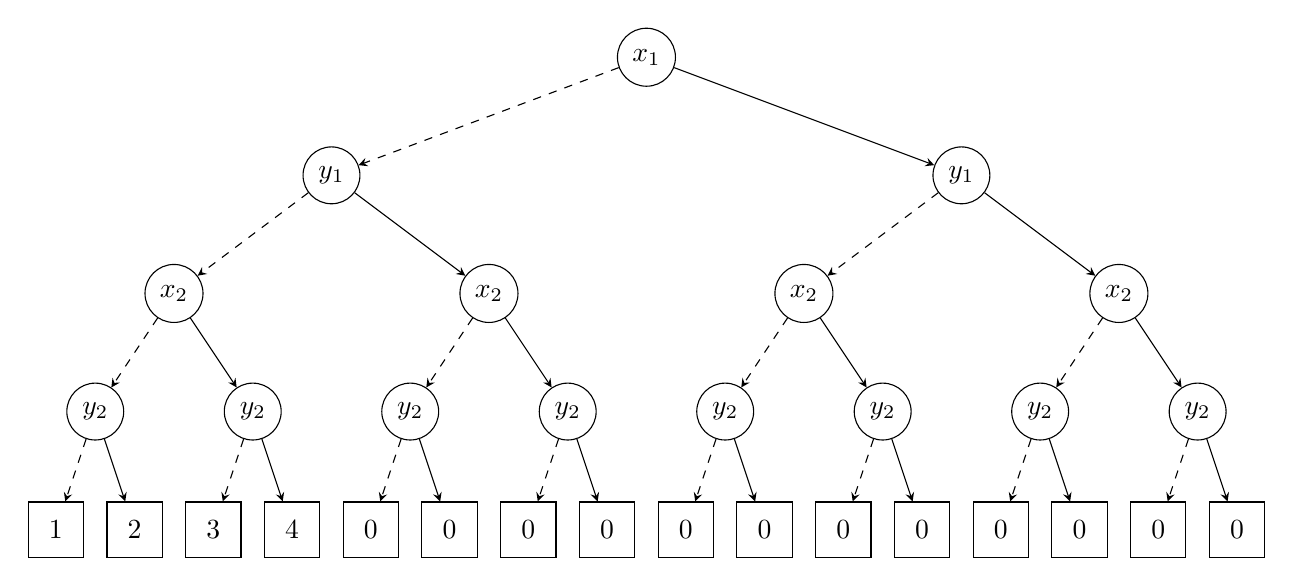
\begin{tikzpicture}[
    level 1/.style={sibling distance=80mm},
    level 2/.style={sibling distance=40mm},
    level 3/.style={sibling distance=20mm},
    level 4/.style={sibling distance=10mm}
    ]
\node[c] {$x_1$}
    child{ node[c]  {$y_1$} edge from parent[zeroarrow]
            child{ node[c] {$x_2$} 
                    child{ node[c] {$y_2$} 
                        child{ node[t] {1}}
                        child{ node[t] {2} edge from parent[onearrow]} 
                    }
                    child{ node[c] {$y_2$} edge from parent[onearrow]
                        child{ node[t] {3} edge from parent[zeroarrow]}
                        child{ node[t] {4}} 
                    }
            }
            child{ node [c] {$x_2$} edge from parent[onearrow]
                    child{ node[c] {$y_2$}  edge from parent[zeroarrow]
                        child{ node[t] {0}} 
                        child{ node[t] {0} edge from parent[onearrow]} 
                    }
                    child{ node[c] {$y_2$} edge from parent[onearrow]
                        child{ node[t] {0} edge from parent[zeroarrow]} 
                        child{ node[t] {0}} 
                    }
            }
    }
    child{ node[c] {$y_1$} edge from parent[onearrow]
            child{ node [c] {$x_2$} edge from parent[zeroarrow]
                    child{ node[c] {$y_2$} 
                        child{ node[t] {0}} 
                        child{ node[t] {0} edge from parent[onearrow]} 
                    }
                    child{ node[c] {$y_2$} edge from parent[onearrow]
                        child{ node[t] {0} edge from parent[zeroarrow]} 
                        child{ node[t] {0}}  
                    }
            }
            child{ node [c] {$x_2$} edge from parent[onearrow]
                    child{ node[c] {$y_2$} edge from parent[zeroarrow]
                        child{ node[t] {0}} 
                        child{ node[t] {0} edge from parent[onearrow]} 
                    }
                    child{ node[c] {$y_2$} edge from parent[onearrow]
                        child{ node[t] {0} edge from parent[zeroarrow]} 
                        child{ node[t] {0}} 
                    }
            }
    }
;
\end{tikzpicture}
    \caption{Vector V represented as an ADD}
    \label{fig:add}
\end{figure*}

The conversion of a matrix to an \gls{add} is similar to that of a vector, but with an additional layer of nodes to represent the rows.
The \gls{add} can however be reduced as shown in \autoref{fig:add_reduced}.
This reduction is done by removing the duplicated terminal nodes, removing the redundant nodes and merging the nodes with the same children.
The techniques for reducing \glspl{add} is the standard reduction techniques used for \glspl{bdd}.
The reduction of the \gls{add} is done to reduce the size of the \gls{add} and to make the operations on the \gls{add} more efficient.
CUDD has built-in functions for reducing the \gls{add}, that follows the standard reduction techniques.

\begin{figure}
    \centering
    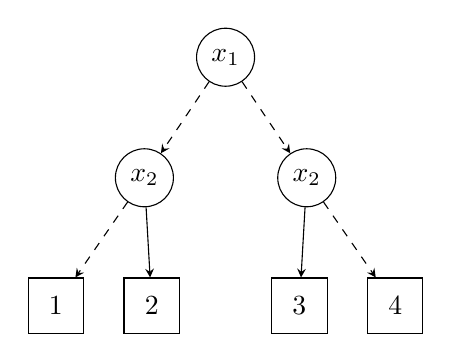
\begin{tikzpicture}[node distance=1cm and 0.5cm]
    \node[c] (x) {$x_1$};
    \node[c] (a) [below left=of x] {$x_2$};
    \node[c] (b) [below right=of x] {$x_2$};
    
    \node[t] (final-1) [below left=of a] {1};
    \node[t] (final-2) [right=of final-1] {2};
    \node[t] (final-4) [below right=of b] {4};
    \node[t] (final-3) [left=of final-4] {3};
    
    \draw[zeroarrow] (x) -- (a);
    \draw[zeroarrow] (a) -- (final-1);
    \draw[onearrow] (a) -- (final-2);
    \draw[zeroarrow] (x) -- (b);
    \draw[onearrow] (b) -- (final-3);
    \draw[zeroarrow] (b) -- (final-4);    
\end{tikzpicture}
    \caption{Reduced ADD of matrix V}
    \label{fig:add_reduced}
\end{figure}

\subsection{CUDD}\label{subsec:cudd}
The Colorado University Decision Diagram (CUDD) library~\cite{somenzi1997cudd} is a powerful tool for implementing and manipulating decision diagrams, including \glspl{bdd} and \glspl{add}. \glspl{add} are compact representations of functions, often used to handle large state spaces symbolically and efficiently.

In this project, the CUDD library stores \glspl{add} and performs operations on them.
Its optimized algorithms and efficient memory management allow us to handle large and complex matrices symbolically, leading to significant performance improvements over traditional methods.

The CUDD library is implemented in C, ensuring high-performance execution, but it also ensures it can be used in C++ programs.

\subsection{Storm}\label{subsec:storm}
Storm is a versatile, open-source probabilistic model checking tool designed to verify the correctness and properties of stochastic models~\cite{hensel2021probabilistic}. It supports a wide range of probabilistic models, including \glspl{hmm}, \glspl{mc} and \glspl{mdp}. Storm allows users to analyze models efficiently by computing various quantitative properties, such as probabilities, expected rewards, or long-run averages.

A key feature of Storm is its ability to represent models symbolically, leveraging data structures like \glspl{bdd} and \glspl{add}. These symbolic representations compactly encode the model's state space and transition structure, enabling efficient manipulation and analysis even for large-scale systems. Storm achieves this by interfacing with the CUDD library, mentioned earlier.

In our implementation, Storm serves as a parser for loading the input models. Specifically, we utilize Storm to convert the model into its \gls{add} representation. This \gls{add} representation provides a compact and hierarchical encoding of the underlying matrices, which can then be used to perform symbolic matrix operations using the CUDD library.

The reason for using Storm lies in it is open-source, which makes it easy to integrate into our project. Storm is designed to handle large and complex models efficiently for model checking.
Therefore the next step in Storm is to calculate the parameters of interest, such as transition probabilities, rewards, or other metrics derived from the model. By performing these computations symbolically within the ADD framework, we achieve a scalable and efficient approach to analyzing stochastic models.


\subsection{Matrix operations using ADDs}\label{subsec:matrix-operations-using-adds}
The matrix operations are implemented using \glspl{add}.
The matrix operations implemented are matrix transpose, matrix addition, matrix multiplication, Hadamard product, Hadamard division, Kronecker product and Khatri-Rao product.

\[
    A = \begin{bmatrix}
            1 & 2 \\
            3 & 4 \\
    \end{bmatrix}
\]

and

\[
    B = \begin{bmatrix}
            5 & 6 \\
            7 & 8 \\
    \end{bmatrix}
\]

are used as examples in the following subsections.

In CUDD the \textit{DdManager} is used to manage the \glspl{add} and the operations on them.
The \textit{DdNode} is used to represent both the \glspl{add} and the variables in the \glspl{add}, that is the row and column indices in the \glspl{add}.

\subsubsection{Matrix Transpose}
The matrix transpose is implemented by swapping the row and column variables in the \gls{add}. Specifically, for each path in the \gls{add} representing an entry $(i, j)$, the roles of the row index 
$i$ and column index $j$ are exchanged. The terminal nodes (values of the matrix entries) remain unchanged.
The transpose of matrix $A$ is:
\[
    A^T = \begin{bmatrix}
              1 & 3 \\
              2 & 4 \\
    \end{bmatrix}
\]

In CUDD the function we use for transposing an \gls{add} is implemented as \textit{Cudd\_addSwapVariables(DdManager * dd, DdNode * f, DdNode ** x, DdNode ** y, int  n )}, where \textit{f} is the \gls{add} to be transposed, \textit{x} and \textit{y} are the set variables to be swapped and \textit{n} is the size of the variables to be swapped.

\subsubsection{Matrix addition}
Matrix addition is implemented by adding the terminal nodes of two \glspl{add} while keeping the structure of the row and column indices consistent. The process involves:
\begin{enumerate}
    \item Traversing the paths of both \glspl{add} simultaneously.
    \item Summing the values at the terminal nodes where the row and column indices match.
\end{enumerate}
The resulting \gls{add} represents the element-wise sum of the two matrices.
The sum of matrices $A$ and $B$ is:
\[
    A + B = \begin{bmatrix}
        6  & 8  \\
        10 & 12 \\
    \end{bmatrix}
\]

In CUDD the function we use for adding two \glspl{add} is implemented as \textit{Cudd\_addApply(DdManager * dd, Cudd\_addPlus(), DdNode * f, DdNode * g)}, where \textit{f} and \textit{g} are the two \glspl{add} to be added and \textit{Cudd\_addPlus()} is the function that is used to add the two \glspl{add}.

\subsubsection{Matrix multiplication}
Matrix multiplication is implemented symbolically using the dot product of the row and column indices. In the \gls{add}:
\begin{enumerate}
    \item For each pair of rows in the first matrix and columns in the second matrix, the corresponding elements are multiplied.
    \item The products are summed along the shared index, combining them into the final terminal nodes of the resulting \gls{add}.
\end{enumerate}
The hierarchical structure of the \gls{add} ensures that only relevant paths are explored, making the operation efficient.
The product of matrices $A$ and $B$ is
\[
    A \times B = \begin{bmatrix}
        19 & 22 \\
        43 & 50 \\
    \end{bmatrix}
\]

%\textit{Cudd\_addMatrixMultiply(DdManager dd, DdNode A, DdNode B, DdNode **z, int nz)}
We use the function \textit{Cudd\_addMatrixMultiply(DdManager dd, DdNode A, DdNode B, DdNode **z, int nz)} in CUDD to multiply two \glspl{add}. 
The function takes two \glspl{add} \textit{A} and \textit{B} to be multiplied as input and returns a pointer to the resulting \gls{add}.
\textit{z} is the set of variables that are dependent on the columns in \textit{A} and the rows in \textit{B}.
\textit{A} is assumed to have the same number of columns as \textit{B} has rows, namely \textit{nz}.

\subsubsection{Hadamard product}\label{subsubsec:hadamard-product}
The Hadamard product is implemented by pairwise multiplication of corresponding terminal nodes in the two \glspl{add}. For each matching row-column index pair $(i, j)$:
\begin{enumerate}
    \item The values from both \glspl{add} are multiplied.
    \item The resulting product is stored in the terminal node of the new \gls{add}.
\end{enumerate}
The structure of the indices remains unchanged.
The Hadamard product of matrices $A$ and $B$ is:

\[
    A \circ B = \begin{bmatrix}
        5  & 12 \\
        21 & 32 \\
    \end{bmatrix}
\]

In CUDD the function we use for Hadamard product is implemented as \textit{Cudd\_addApply(DdManager * dd, Cudd\_addTimes(), DdNode * f, DdNode * g)}, where \textit{f} and \textit{g} are the two \glspl{add} to be multiplied and \textit{Cudd\_addTimes()} is the function that is used to multiply the two \glspl{add} elementwise.

\subsubsection{Hadamard division}
The Hadamard division is implemented as Hadamard product, but with division instead of multiplication. See~\autoref{subsubsec:hadamard-product} for more details.
The Hadamard division of matrices $A$ and $B$ is

\[
    A \oslash B = \begin{bmatrix}
        0.2    & 0.3333 \\
        0.4286 & 0.5    \\
    \end{bmatrix}
\]

The Hadamard division is implemented by \textit{Cudd\_addApply(DdManager * dd, Cudd\_addDivide(), DdNode * f, DdNode * g)}, where \textit{f} and \textit{g} are the two \glspl{add} to be divided and \textit{Cudd\_addDivide()} is the function that is used to divide the two \glspl{add} elementwise.

\subsubsection{Kronecker product}
The Kronecker product is implemented by expanding the indices and terminal nodes of the two matrices symbolically, with the resulting \gls{add} having the dimensions of the sum of the dimensions of the two matrices. 
The Kronecker product is a generalization of the outer product, where each element of the first matrix is multiplied by the second matrix as a whole.
For each entry $(i, j)$ in the first matrix with value $a$, the second matrix $B$ is multiplied by $a$, and the indices are adjusted:
\begin{enumerate}
    \item The row and column indices of $B$ are shifted based on $i$ and $j$ of $A$.
    \item The resulting values are stored in a new \gls{add}.
\end{enumerate}
The Kronecker product of matrices $A$ and $B$ is

\[
    A \otimes B = \begin{bmatrix}
        5  & 6  & 10 & 12 \\
        7  & 8  & 14 & 16 \\
        15 & 18 & 20 & 24 \\
        21 & 24 & 28 & 32 \\
    \end{bmatrix}
\]

\subsubsection{Khatri-Rao product}
The Khatri-Rao product is implemented by combining rows of the first matrix with corresponding rows of the second matrix. For each row index $i$:
\begin{enumerate}
    \item The elements of row $i$ in the first matrix are multiplied element-wise with the entire row $i$ in the second matrix.
    \item The resulting row is constructed symbolically within the \gls{add}.   
\end{enumerate}
The Khatri-Rao product of matrices $A$ and $B$ is

\[
    A \bullet B = \begin{bmatrix}
        5  & 6  & 10 & 12 \\
        21 & 24 & 28 & 32 \\
    \end{bmatrix}
\]
The resulting \gls{add} has the dimensions of sum of the dimensions of the two matrices, as in the Kronecker product.

% \subsubsection{Matrix scalar}
% Matrix scalar is implemented by multiplying each element in the matrix by a scalar value.
% The scaling of matrix $A$ by a factor of 2 is
% \[
% 2 \times A = 2 \times \begin{bmatrix}
%     1 & 2 \\
%     3 & 4 \\
% \end{bmatrix} = \begin{bmatrix}
%     2 & 4 \\
%     6 & 8 \\
% \end{bmatrix}
% \]

% The \gls{add} representation of the scaled matrix is shown in Figure \ref{fig:add_scaling}.
% \begin{figure}
%     \centering
%     \begin{tikzpicture}[
% level 1/.style={sibling distance=20mm},
% level 2/.style={sibling distance=10mm},
% level 3/.style={sibling distance=10mm}
% ]
% \node[c] {$x_1$}
%     child{ node[c]  {$y_1$} edge from parent[zeroarrow]
%             child{ node[t] {2} 
%             }
%             child{ node [t] {4} edge from parent[onearrow]
%             }
%     }
%     child{ node[c] {$y_1$} edge from parent[onearrow]
%         child{ node[t] {6} edge from parent[zeroarrow]
%         }
%         child{ node[t] {8} edge from parent[onearrow]}
%     }
% ;
%     \end{tikzpicture}
%     \caption{Scaling of matrix A by a factor of 2}
%     \label{fig:add_scaling}
% \end{figure}

    \section{Experiments}\label{sec:experiments}
In this section, we describe the experiments conducted to evaluate the proposed symbolic implementation of the Baum-Welch algorithm in CuPAAL. 
The experiments are designed to compare CuPAAL with two other implementations: Jajapy, the original matrix-based implementation, and SUDD, a hybrid symbolic and matrix-based implementation.
The experiments are conducted to answer the following research questions:

\begin{itemize}
    \item \textbf{Question 1:} How does the symbolic CuPAAL implementation compare to Jajapy and SUDD in terms of parameter estimation accuracy and runtime?
    \item \textbf{Question 2:} How does the scalability of the symbolic CuPAAL implementation compare to Jajapy and SUDD as the number of model states increases?
\end{itemize}

These questions evaluate both the computational efficiency and accuracy of the symbolic implementation in CuPAAL. The insights gained will highlight the strengths and potential trade-offs of symbolic approaches to the Baum-Welch algorithm.

\subsection{Experimental Setup}
Two experiments are conducted to address the research questions.

\textbf{Experiment 1: Parameter Estimation Accuracy.} This experiment compares the runtime, parameter estimation accuracy, and convergence properties of the Baum-Welch implementations.

\textbf{Experiment 2: Scalability.} This experiment evaluates how each implementation scales with an increasing number of model states.
We conduct two experiments to evaluate the proposed method.

All experiments are conducted on a machine with INSERT\_SPECS\_FOR\_MACHINE\_HERE.
The experiments are all run 10 times to ensure consitency, with the results averaged to account for any variance in runtime and estimation accuracy.
We use the following implementations for the experiments:
\begin{itemize}
    \item \textbf{Jajapy}: The original implementation of the Baum-Welch algorithm~\cite{reynouard2023jajapy}.
    \item \textbf{SUDD}: The SUDD implementation of the Baum-Welch algorithm~\cite{p7}.
    \item \textbf{SUDD\_log}: The SUDD implementation of the Baum-Welch algorithm using a logsemiring for numerical stability.
    \item \textbf{CuPAAL}: The symbolic implementation of the Baum-Welch algorithm proposed in the paper.
\end{itemize}

The chosen implementations represent a progression from fully matrix-based to hybrid, to fully symbolic approaches, providing a comprehensive comparison of methodologies.

\subsection{Experiment 1: Parameter Estimation Accuracy}
The first experiment measures runtime, accuracy, and convergence properties of the Baum-Welch algorithm across implementations.
We use the following models for the experiment:
\begin{itemize}
    \item FIND THE MODELS USED IN THE EXPERIMENT HERE
\end{itemize} 
We generate observation sequences from each model and use the Baum-Welch algorithm to estimate the parameters of the model. 
We make 100 observations with a sequence length of 30 for each model.

The experiment is made with the following steps:
\begin{enumerate}
    \item Load the model.
    \item Generate an observation sequence from the model.
    \item Generate initial parameters.
    \item Use each implementation of the Baum-Welch algorithm to estimate model parameters, recording parameter estimates and runtime.
    \item Repeat steps 2 to 4 ten times, averaging results.
    \item Compare the estimated parameters with the true parameters.
\end{enumerate}
All the implementations are tested with the same observation sequences and initial parameters to ensure a fairness.

We use the following evaluation metrics to compare the Baum-Welch implementations:
\begin{itemize}
    \item \textbf{Relative parameter error}: Accuracy of the estimated parameters compared to the true parameters.
    Calculated as $\frac{|r - e|}{e}$, where $r$ is the real parameter and $e$ is the expected value of the parameter.
    \item \textbf{Relative formula error}: Accuracy of the estimated formulas using Storm by providing estimated parameters and checking the formula error.
    \item \textbf{Runtime}: Total computation time for parameter estimation.
    \item \textbf{Iterations}: The number of iterations required to converge.
\end{itemize}

We use the relative parameter error and relative formula error to compare the accuracy of the estimated parameters and formulas across implementations, this will give us an idea of how accurate the Baum-Welch algorithm is in each implementation.

We use the runtime to compare the computational efficiency of the Baum-Welch algorithm across implementations.
We use the number of iterations to ensure that all implementations have converged to the same solution, meaning that the comparison is fair.

The results are presented in tables to facilitate a direct comparison of performance across models and between implementations.

\subsection{Scalability experiment}
The second experiment assesses scalability by increasing the number of states in a model \textit{MODEL NAME HERE} from 2 to 10,000. 
Observation sequences are generated with the same settings as Experiment 1, and the process is repeated as follows:

\begin{enumerate}
    \item Load the model.
    \item Generate an observation sequence from the model.
    \item Generate initial parameters.
    \item Use each implementation of the Baum-Welch algorithm to estimate model parameters, recording runtime.
    \item Repeat steps 2 to 4 ten times, averaging results.
    \item Increase the number of states in the model and repeat the entire process.
\end{enumerate}

Scalability is evaluated by examining runtime trends as model size increases. 
This gives insight into how each implementation scales with larger models and is critical for understanding the practical applicability of symbolic versus matrix-based implementations for large-scale problems.

Results will be visualized using plots to illustrate trends and highlight differences in scalability between implementations.


    \printglossary[type=\acronymtype]

    \printbibliography

    \appendices % You can use \appendix if you only have a single appendix
    %! Author = Runge
%! Date = 29-12-2023

\section{Compiling in draft}\label{sec:compiling-in-draft}
You can also compile the document in draft mode.
This shows todos, and increases the space between lines to make space for your supervisors feedback.


\end{document}
